% Created 2024-02-04 dim. 17:00
% Intended LaTeX compiler: pdflatex
\documentclass[11pt]{article}
\usepackage[utf8]{inputenc}
\usepackage[T1]{fontenc}
\usepackage{graphicx}
\usepackage{longtable}
\usepackage{wrapfig}
\usepackage{rotating}
\usepackage[normalem]{ulem}
\usepackage{amsmath}
\usepackage{amssymb}
\usepackage{capt-of}
\usepackage{hyperref}
\usepackage[T1]{fontenc}
\usepackage{lmodern}
\author{J.-M. Chauvet}
\date{\today}
\title{Memory GAPS: Are LLMs Tulving-Complete?}
\hypersetup{
 pdfauthor={J.-M. Chauvet},
 pdftitle={Memory GAPS: Are LLMs Tulving-Complete?},
 pdfkeywords={},
 pdfsubject={},
 pdfcreator={Emacs 28.2 (Org mode 9.6.3)}, 
 pdflang={English}}
\usepackage{natbib}
\begin{document}

\maketitle

\section*{Abstract}
\label{sec:orgcc84017}
\section*{Introduction}
\label{sec:org0f17253}
In his groundbreaking studies of memory, Endel Tulving (1927-2023) noted that "one of the most compelling and salient characteristics of remembering of past events is the individual's subjective awareness of remembering" \citep{Tulving1983}. In order to include the rememberer's recollective experience into the critical constructs in the conceptualization of remembering, Tulving suggested an "overall pretheoretical framework", called the \emph{General Abstract Processing System} or GAPS. This paper investigates whether the GAPS also provides insights when the subject is no longer human but a Large Language Model (LLM).

Tulving championed the distinction of \emph{episodic} from \emph{semantic} memory, successfully arguing that being functionnally different, they represent separate but related systems. Both are placed on the same side of the cognitive division between \emph{declarative memory} (as episodic and semantic information can be expressed through language--e.g. repairing a bicycle) on the one hand, and \emph{skills} (which can be observed only in behavior--e.g. riding a bicycle) on the other.

In Tulving's framework, a single act of remembering forms the unit of human episodic memory. Remembering is a process that begins with the witnessing or experiencing of an episode and ends with its recollective experience or with the conversion of the remembered information into some other form, or both. The GAPS specifies so called \emph{elements} of remembering and their interrelations in order to decompose this process.

The GAPS distinguishes two kinds of elements: observable events and hypothetical constructs (processes and states); and it divides elements into two categories: elements of encoding and elements of retrieval.

\begin{figure}[htbp]
\centering
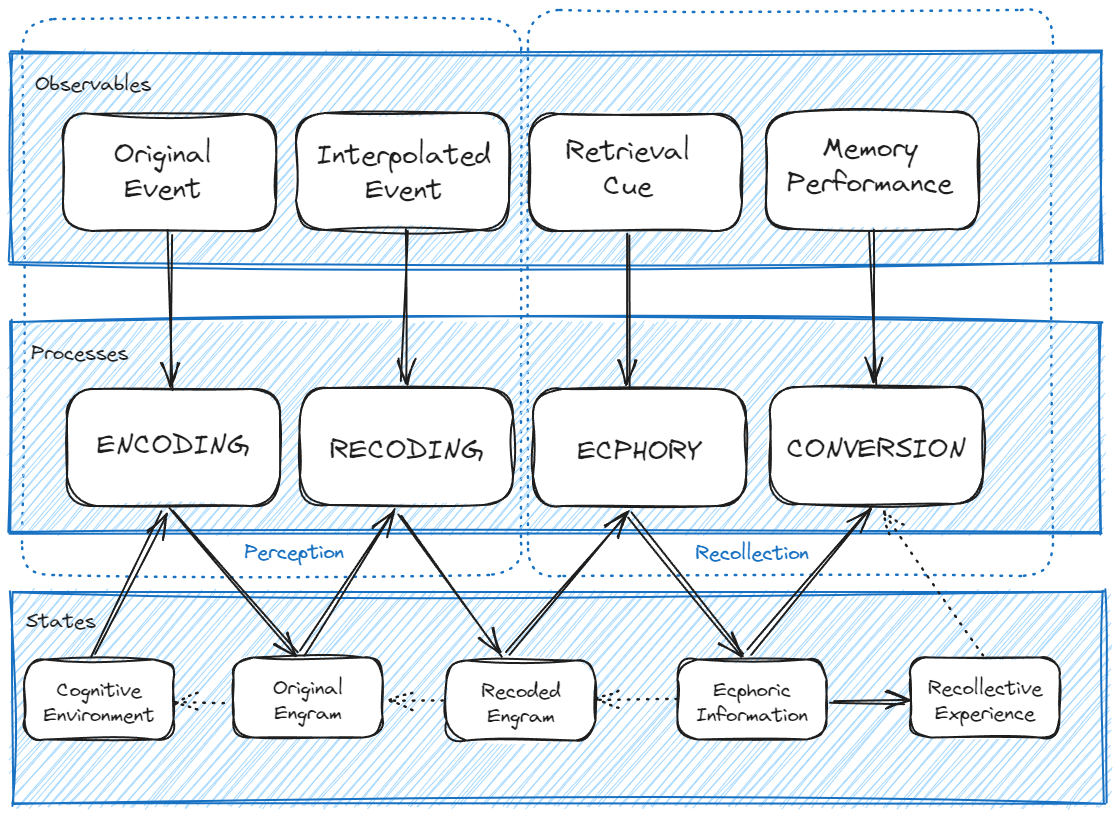
\includegraphics[width=.9\linewidth]{ElementsOfRemembering-rev.png}
\caption{\label{fig:orgd9de8b9}\textbf{The GAPS: Elements of Episodic Memory and their Relations.} The element of encoding is a process that converts the information about an experienced event or episode (in a particular setting, at a particular time) into an \emph{engram} or memory trace. The central element of the retrieval processes \emph{ecphoric} information, a synergistic product of the engram and the retrieval cue, which calls on both episodic and semantic information. Source: \citep[Ch. 7, Fig. 7-1, p. 135]{Tulving1983}.}
\end{figure}

Of particular interest to this study of applicability of the GAPS framework to LLM are the possible transpositions of engram and ecphoric information in the domain of generative AI. In his seminal book, Tulving offers a very broad definition of engrams as "the product of encoding", "conditions for recollection of the experienced event", or "differences between the state of the memory system before and after encoding", the latter closed to the original introduction of the terms by Richard Semon (1859--1918)) "to represent the enduring changes brought about by the energetic effect of stimuli in the organism" \citep{SCHACTER1978721,Semon}. Note that the nature of the changes are unknown, but the term became known to psychology research through the work of Karl Lashley (1890--1958) concluding, amongst other experimental results on neural mechanisms in learning and memory that "there is no demonstrable localization of memory trace" \citep{lashley1950search}.

Similarly inspired by Semon, Tulving suggested the terms \emph{ecphory} and \emph{ecphoric information} to designate the process that brings (i) the relevant information in the retrieval environment into interaction with  (ii) the original or recoded engram, and the output of this process. Such ecphoric information determines the particulars of recollective experience, in the next phase of remembering: conversion.

\section*{Results}
\label{sec:org97969f3}
\section*{Discussion}
\label{sec:org9544f30}
\section*{Methods}
\label{sec:org9aa4c74}
We transpose the 'direct comparison' experiment, between recognitin and recall, described in \citep[Chapter 14]{Tulving1983} to LLM subjects.
\section*{References}
\label{sec:org097a374}

\bibliographystyle{agsm}
\bibliography{c:/Users/chauv/Documents/NEWNEWAI/newnewai}

\section*{Acknowledgements}
\label{sec:org7f045cd}
\section*{Author information}
\label{sec:org5faadc3}
\section*{Ethics declarations}
\label{sec:org1e1c8bc}
\section*{Additional information}
\label{sec:org907a432}
\section*{Electronic supplementary material}
\label{sec:org2850bf3}
\section*{Rights and permissions}
\label{sec:orgcbe19a4}
\section*{About this article}
\label{sec:orgdfe8963}
\section*{Further reading}
\label{sec:orgcdf3069}
\section*{Comments}
\label{sec:org92cff51}
\end{document}